\documentclass[a4paper,12pt]{article}
\usepackage[UTF8]{ctex} % 支持中文
\usepackage{geometry}
\usepackage{graphicx}   % 支持图片插入
% 如果图片缺失，使用占位框，避免编译失败
\newcommand{\safeincludegraphics}[2][]{%
    \IfFileExists{#2}{\includegraphics[#1]{#2}}{\fbox{\parbox[c][0.18\textheight][c]{0.9\linewidth}{\centering 图片缺失: #2}}}%
}
\usepackage{float}      % 图片位置控制
\usepackage{listings}   % 代码块支持
\usepackage{xcolor}     % 颜色支持
\usepackage{amsmath}    % 数学公式

% 设置页面边距
\geometry{left=2.5cm,right=2.5cm,top=2.5cm,bottom=2.5cm}

% 设置MATLAB代码样式
\lstset{
    language=Matlab,
    basicstyle=\scriptsize\ttfamily,
    keywordstyle=\color{blue},
    stringstyle=\color{purple},
    commentstyle=\color{green!60!black},
    numbers=left,
    numberstyle=\tiny\color{gray},
    stepnumber=1,
    frame=single,
    breaklines=true,
    backgroundcolor=\color{gray!5},
    showstringspaces=false,
    captionpos=b
}

\title{\textbf{模拟电路实验 Lab 4 实验报告}}
\author{姓名: 黄瑞颀 \quad 学号: 2024531064}
\date{\today}

\begin{document}

\maketitle

\section{参数设置与串联电阻 $R_s$ 计算}

根据 Lab 2 测得的 $I-V$ 数据，选取大电流线性区域（0.25mA 至 0.6mA 附近），通过线性拟合计算二极管的体电阻 $R_s$。

\subsection{MATLAB 处理代码}
\begin{lstlisting}[title=计算 Rs]
clear; clf;
filename = "PN数据.csv"; 

if isfile(filename)
    data_table = readtable(filename); 
    V_iv = table2array(data_table(:,1))'; 
    I_iv = table2array(data_table(:,2))';
    
    % 选取线性区域 (第55-59行)
    start_row = 55;  
    end_row = 59;    
    V_part = V_iv(start_row:end_row);
    I_part = I_iv(start_row:end_row);
    
    p = polyfit(V_part, I_part, 1); 
    Rs = 1 / p(1); 
    
    fprintf('电阻 Rs = %.4f 欧姆\n', Rs);
    
    figure(1);
    plot(V_iv(start_row:end_row), I_iv(start_row:end_row), 'bo', 'LineWidth', 2); hold on;
    y_fit = polyval(p, V_iv(start_row:end_row));
    plot(V_iv(start_row:end_row), y_fit, 'g-', 'LineWidth', 2);
    title(['Rs 计算: ' num2str(Rs) ' Ohms']);
    grid on;
else
    fprintf('未找到数据文件\n');
end
\end{lstlisting}

\subsection{计算结果与图像}
\begin{figure}[H]
    \centering
    % 请将 MATLAB Figure 1 保存为 fig_rs.png 并放在同一目录下
    % 如果没有图片，可以使用 demo 占位符
    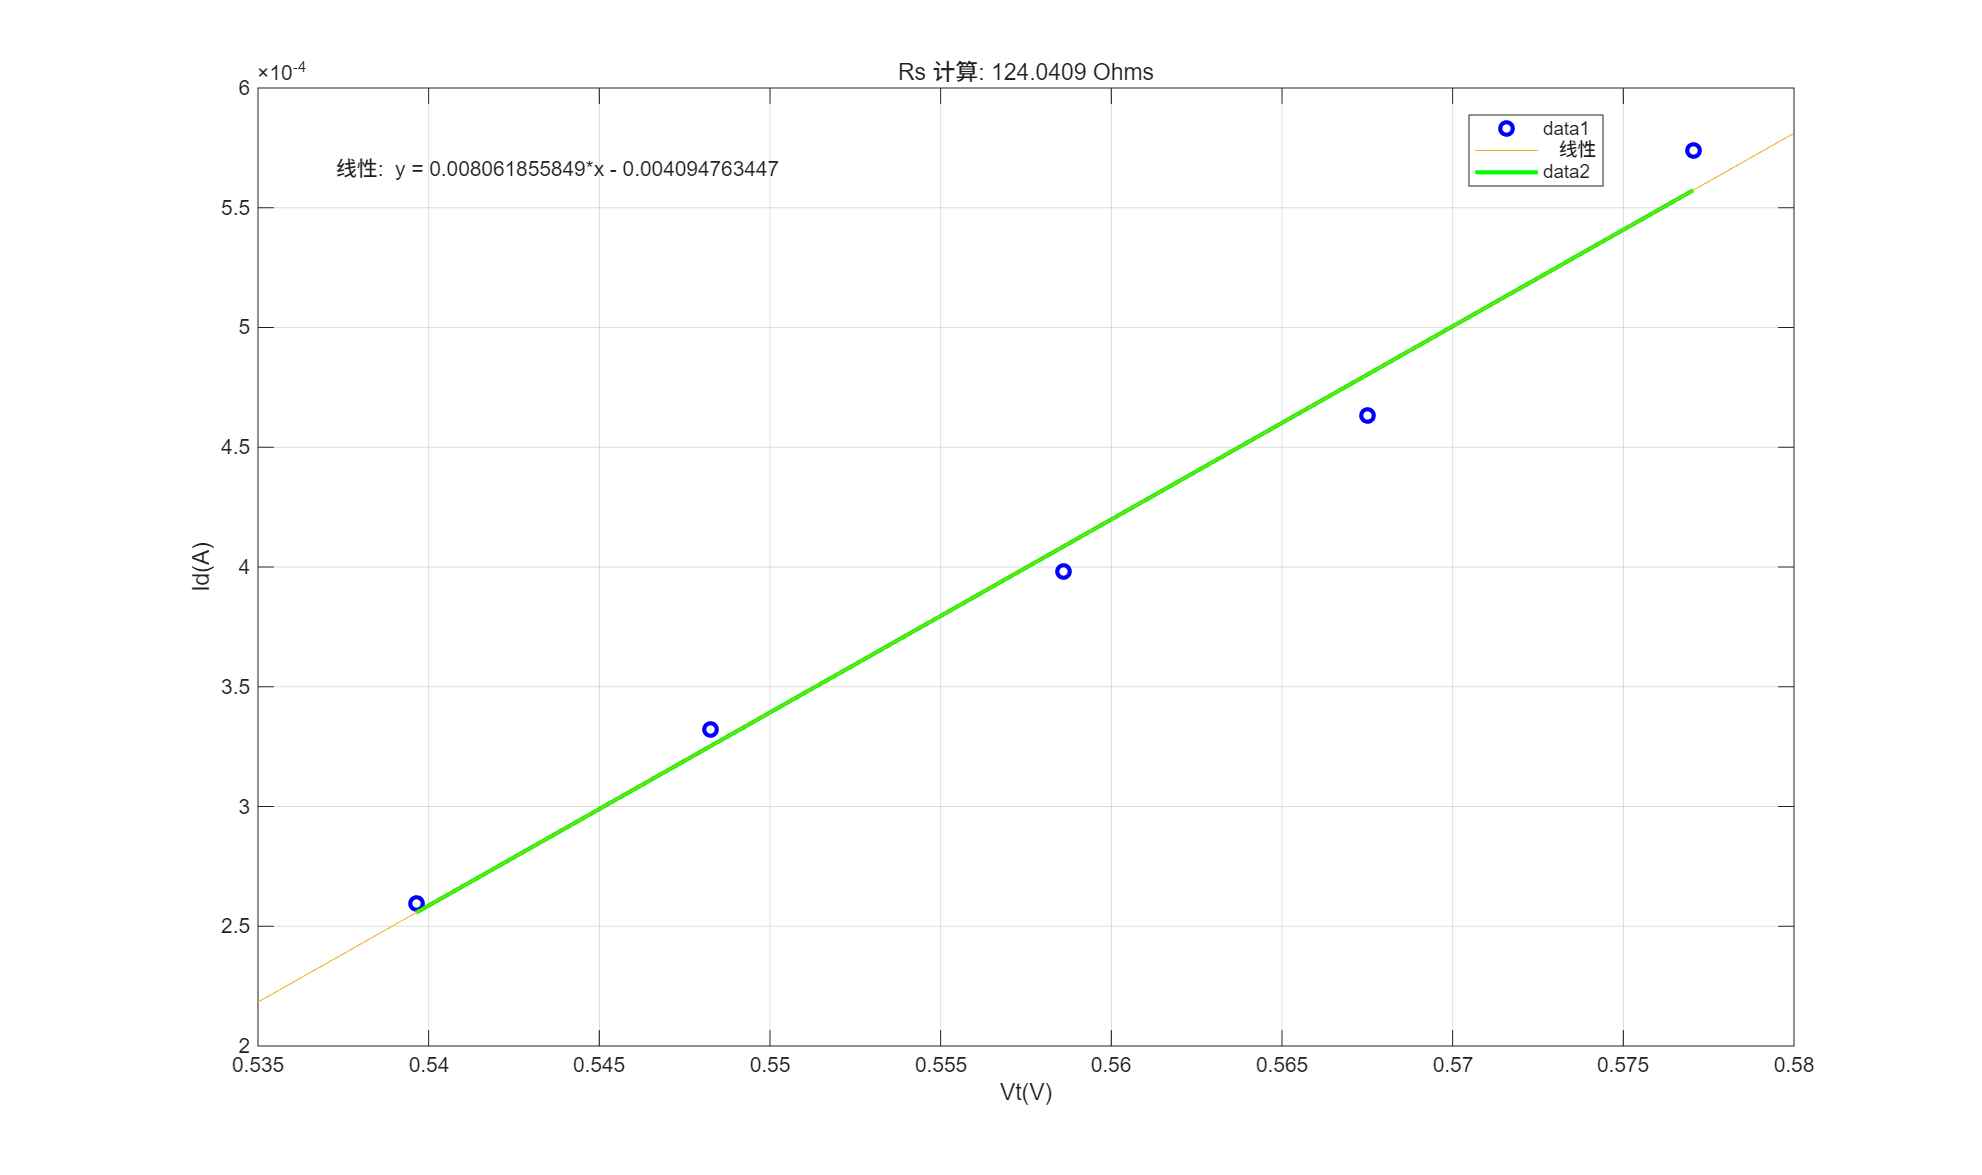
\includegraphics[width=0.7\textwidth]{fig_rs.png} 
    \caption{Rs 线性拟合图}
    \label{fig:rs}
\end{figure}

\begin{itemize}
    \item 计算得到$R_s=\frac{1}{k}\approx 124.0409 \Omega$
\end{itemize}

\section{Multisim 仿真与数据记录}

搭建 RLC 串联谐振电路，调节直流偏置电压 $V_d$。
\textbf{注意：} 本次实验仿真中，为了获得更清晰的高频谐振特性，电感值设定为 \textbf{10 mH (0.01 H)}。

\begin{figure}[H]
    \centering
    % 请插入 Multisim 电路图或 AC Sweep 扫描结果截图
    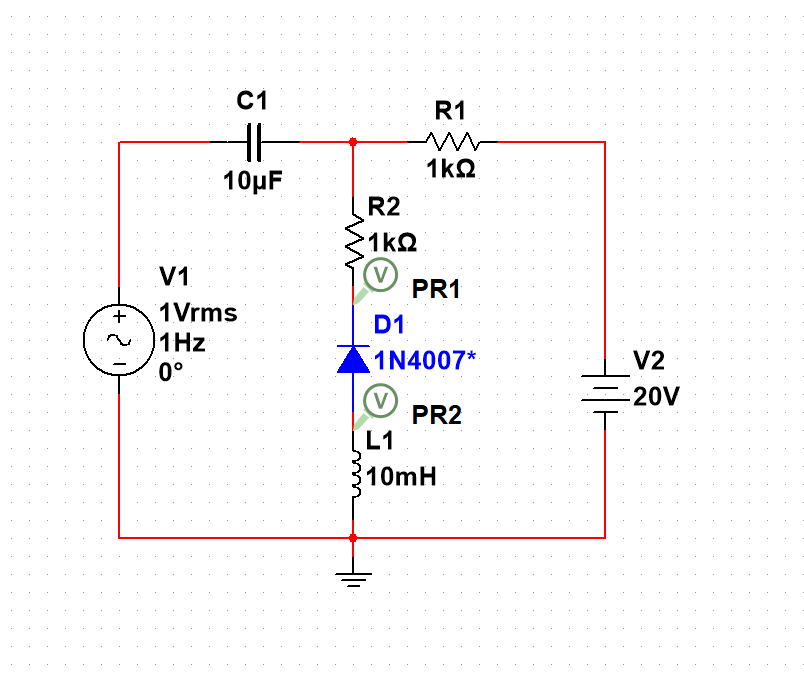
\includegraphics[width=0.5\textwidth]{fig_circuit.png}
    \caption{Multisim 仿真电路}
    \label{fig:multisim}
\end{figure}

% AC Sweep 结果（不同偏压）
\begin{figure}[H]
    \centering
    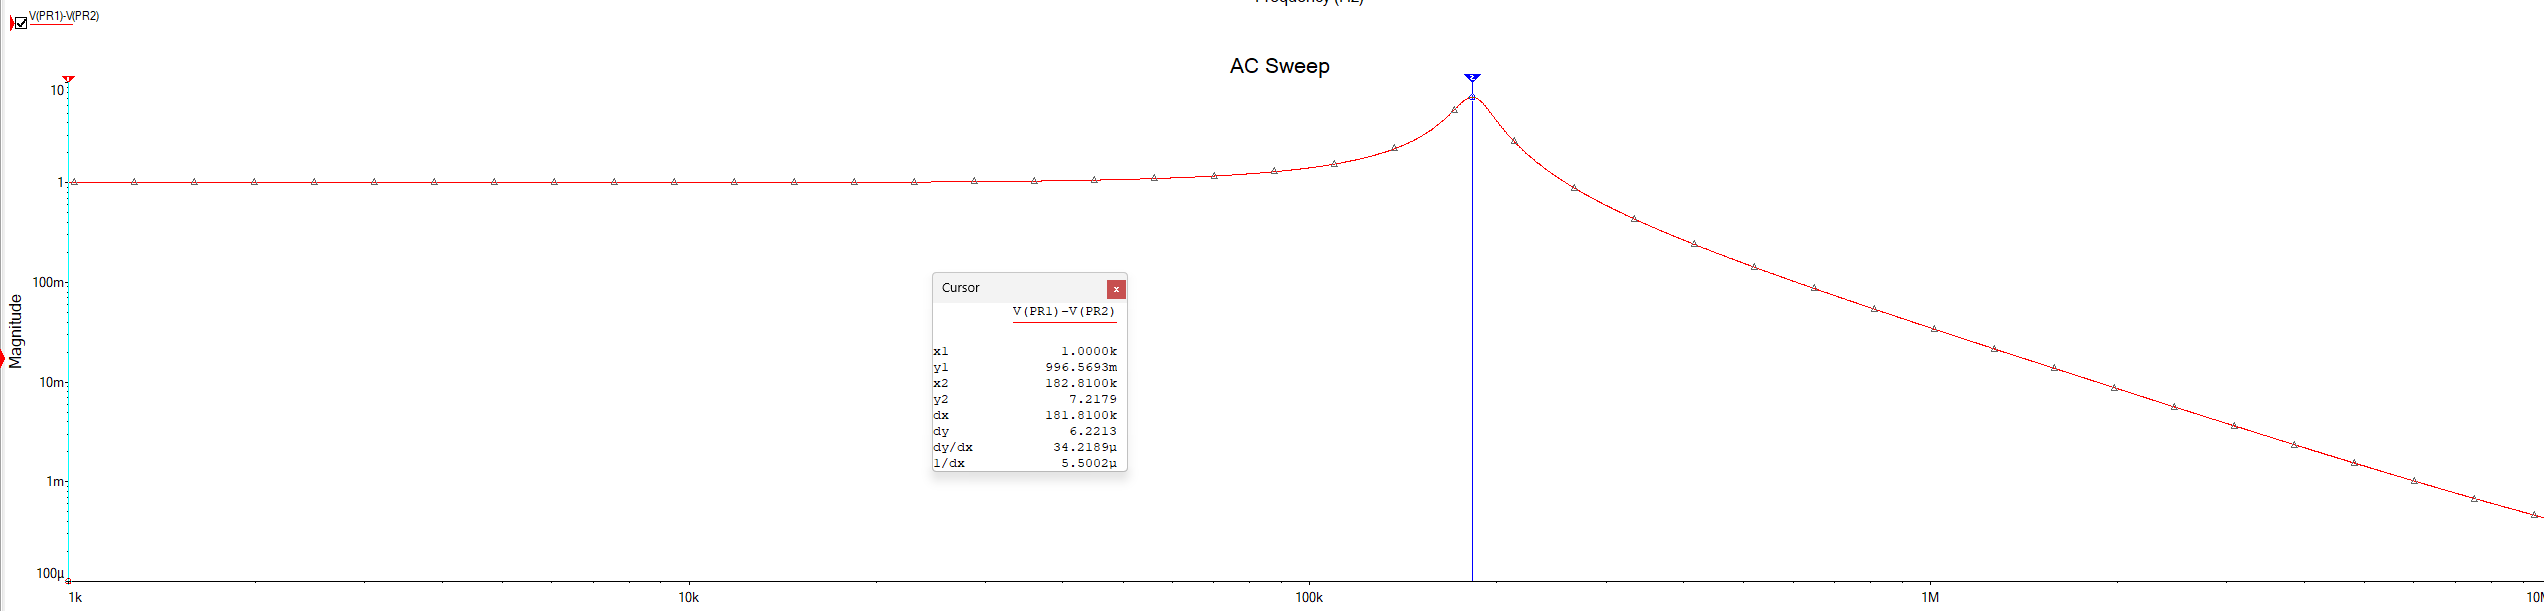
\includegraphics[width=1.0\textwidth]{fig_ac_0p3.png}
    \caption{AC Sweep，偏压 $V_d = 0.3\,\mathrm{V}$}
    \label{fig:ac_0p3}
\end{figure}

\begin{figure}[H]
    \centering
    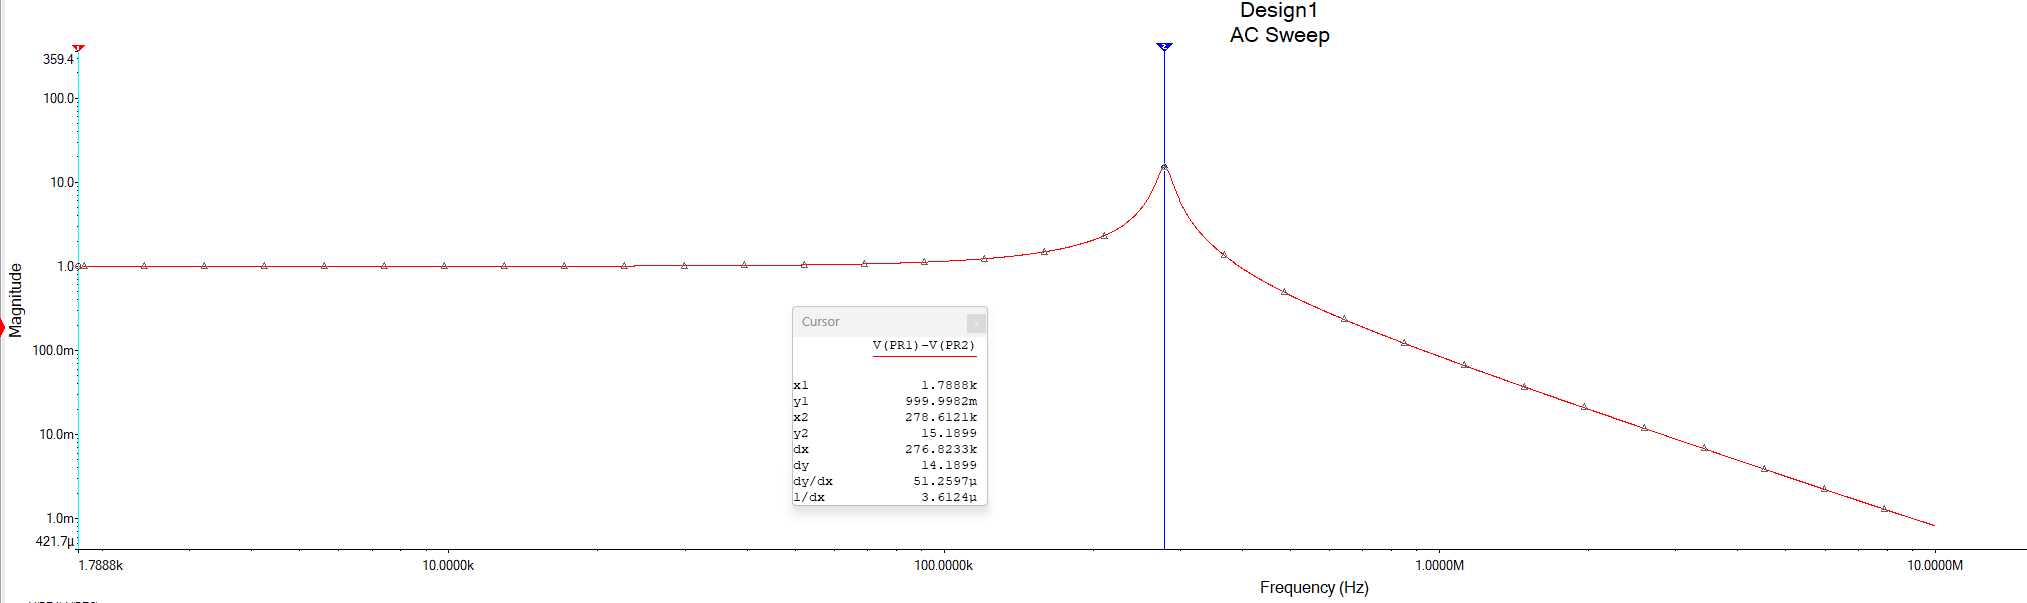
\includegraphics[width=1.0\textwidth]{fig_ac_1.png}
    \caption{AC Sweep，偏压 $V_d = 1\,\mathrm{V}$}
    \label{fig:ac_1}
\end{figure}

\begin{figure}[H]
    \centering
    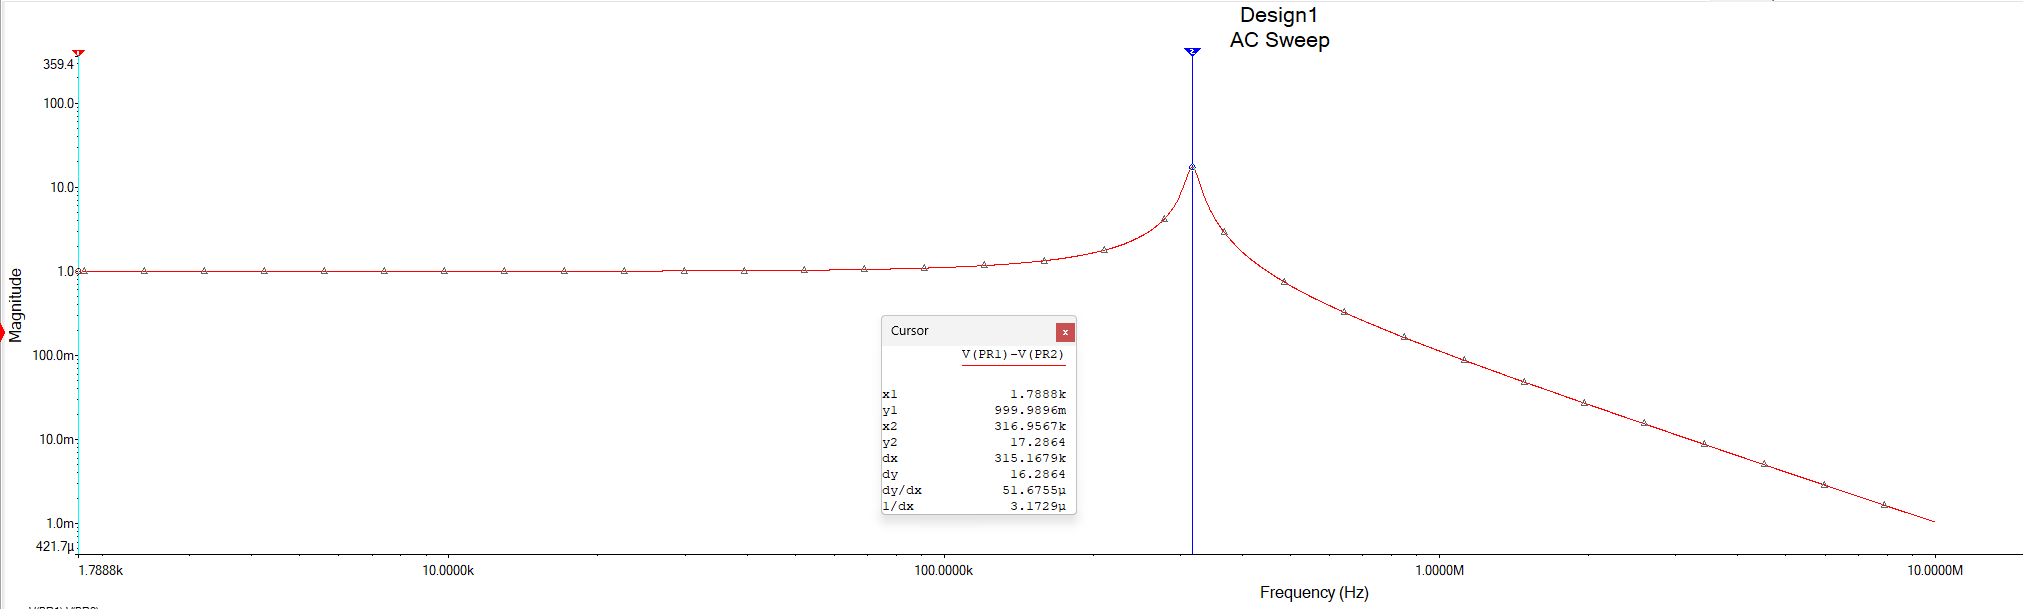
\includegraphics[width=1.0\textwidth]{fig_ac_2.png}
    \caption{AC Sweep，偏压 $V_d = 2\,\mathrm{V}$}
    \label{fig:ac_2}
\end{figure}

\begin{figure}[H]
    \centering
    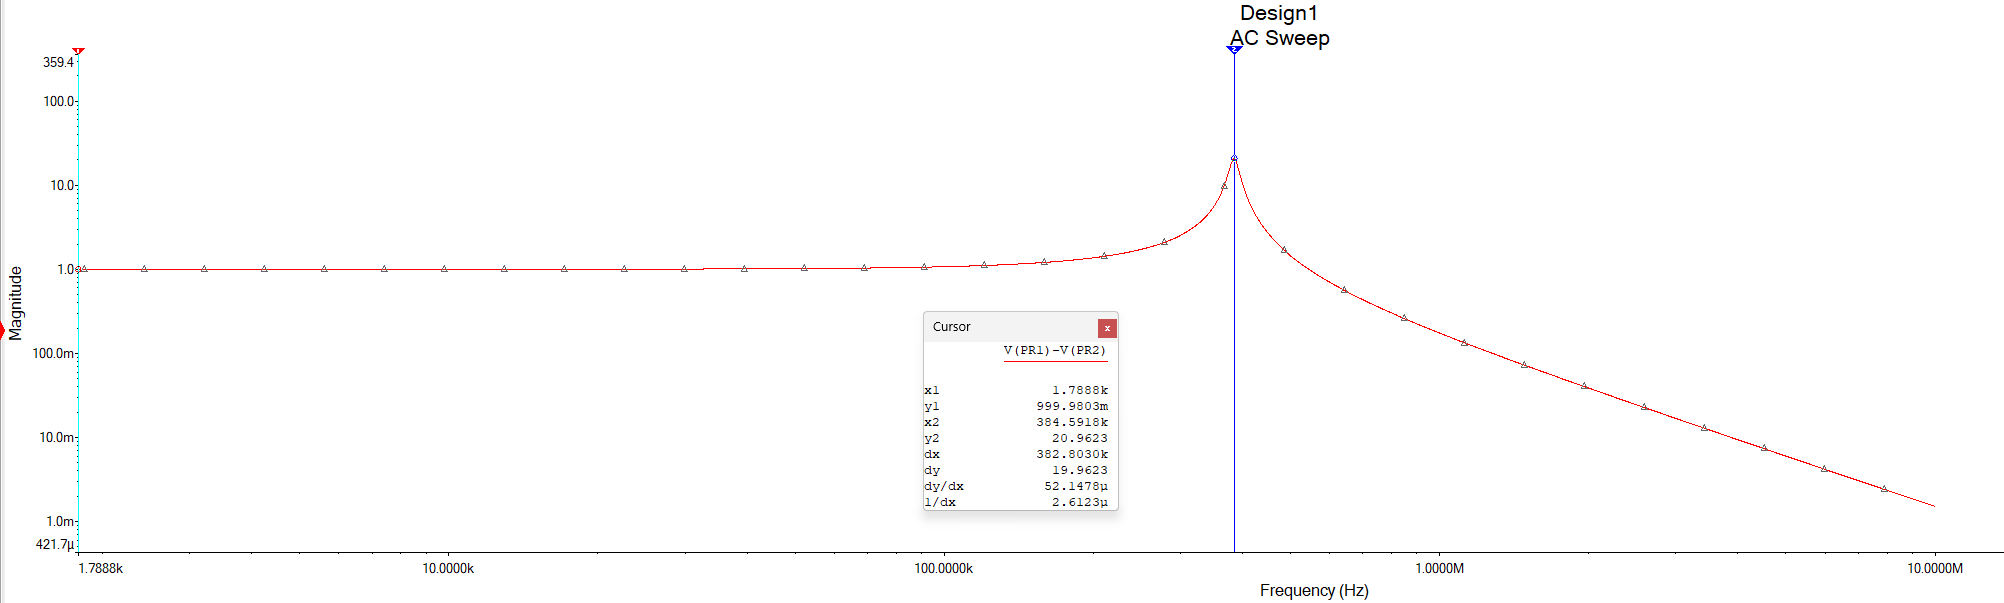
\includegraphics[width=1.0\textwidth]{fig_ac_4.png}
    \caption{AC Sweep，偏压 $V_d = 4\,\mathrm{V}$}
    \label{fig:ac_4}
\end{figure}

\begin{figure}[H]
    \centering
    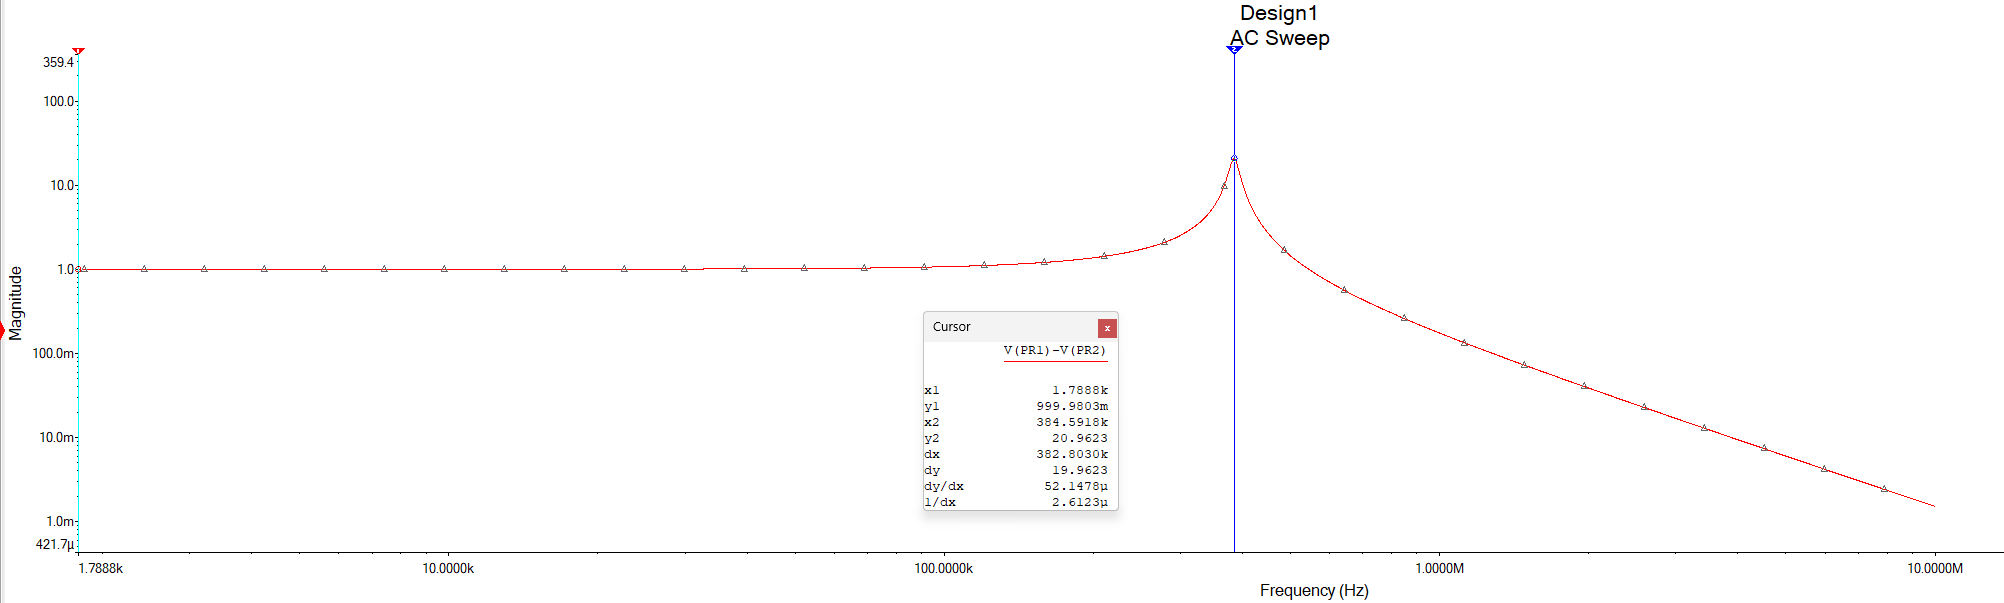
\includegraphics[width=1.0\textwidth]{fig_ac_5.png}
    \caption{AC Sweep，偏压 $V_d = 5\,\mathrm{V}$}
    \label{fig:ac_5}
\end{figure}

\begin{figure}[H]
    \centering
    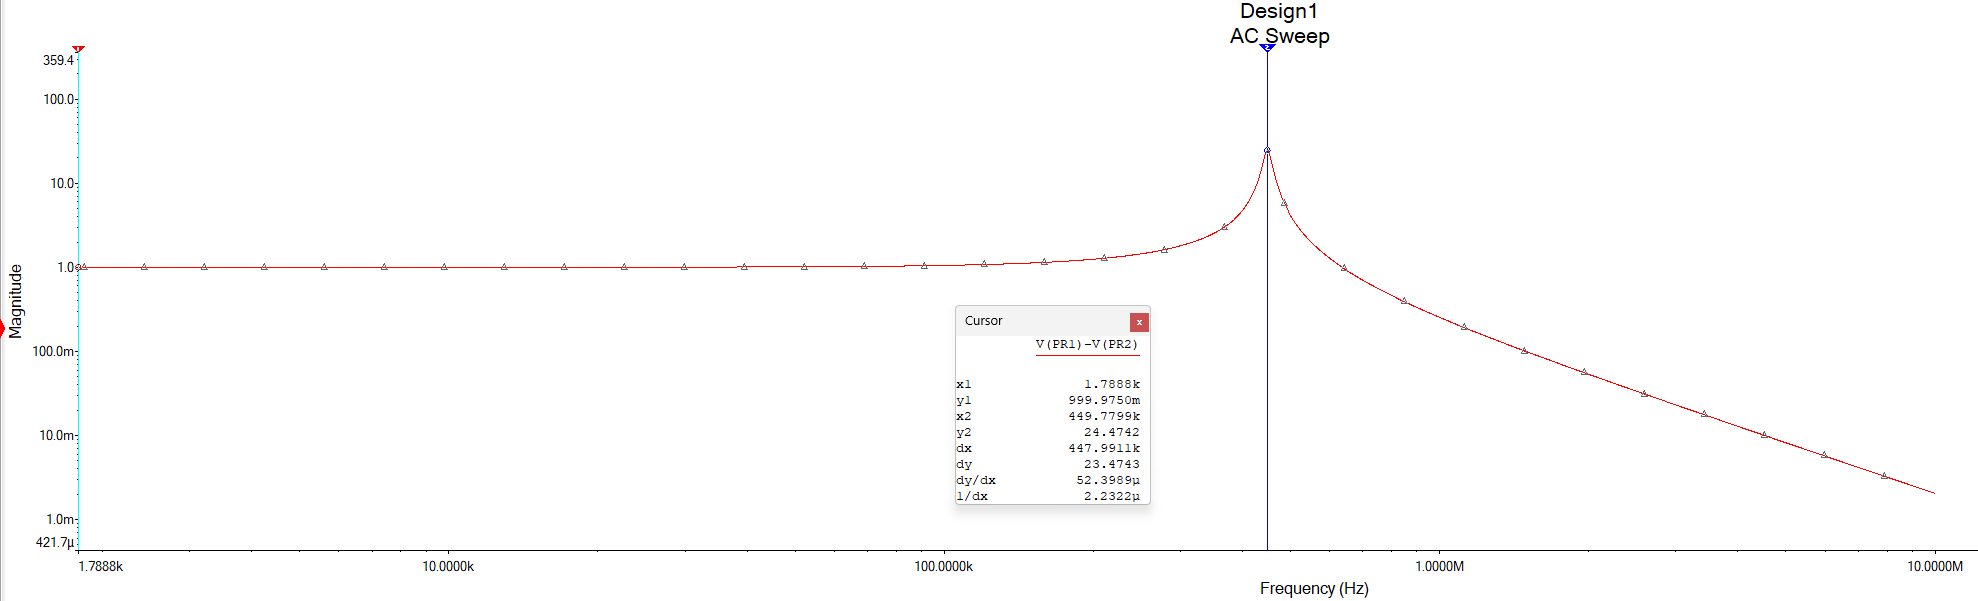
\includegraphics[width=1.0\textwidth]{fig_ac_10.png}
    \caption{AC Sweep，偏压 $V_d = 10\,\mathrm{V}$}
    \label{fig:ac_10}
\end{figure}

\begin{figure}[H]
    \centering
    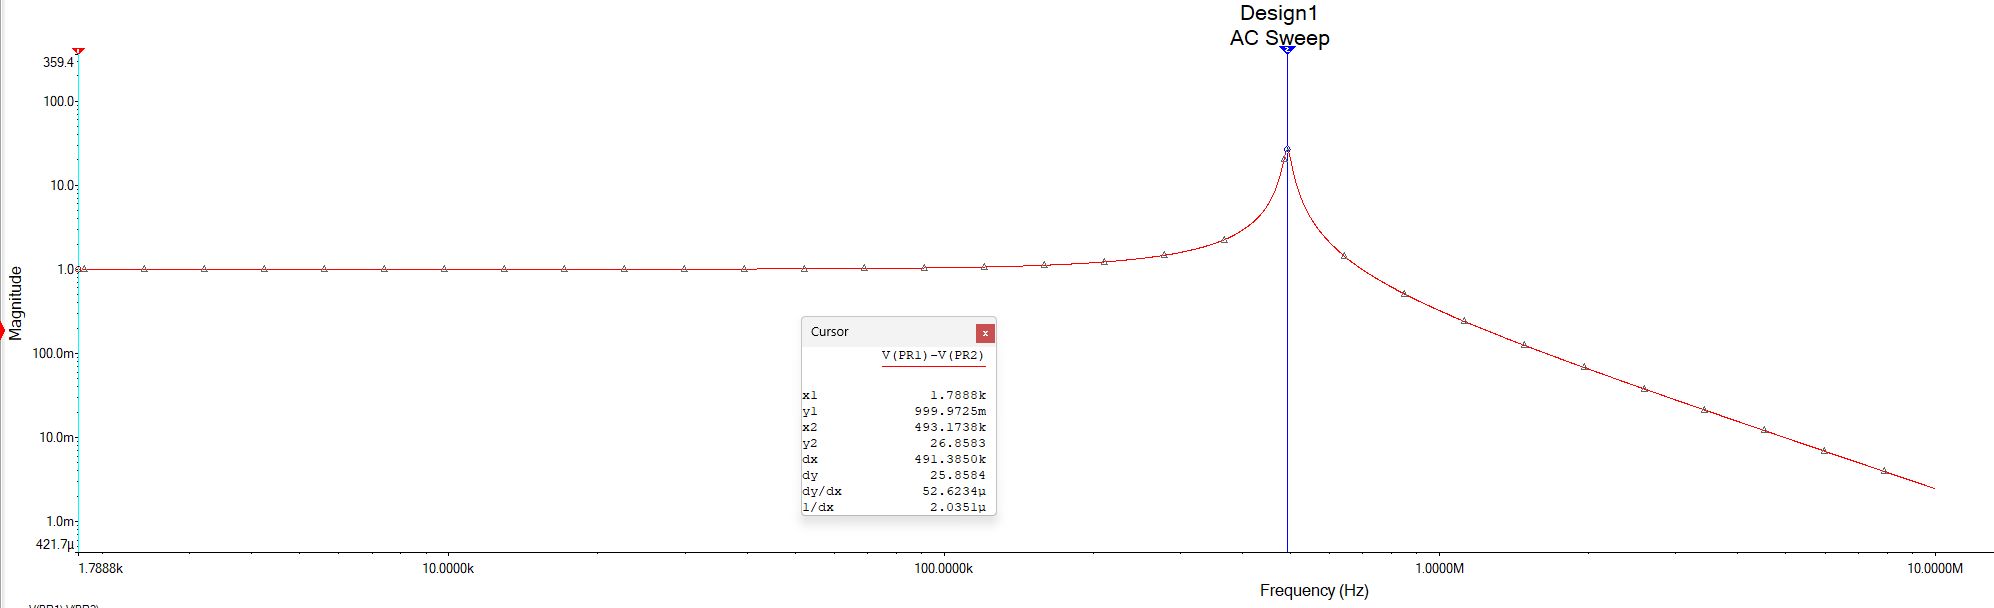
\includegraphics[width=1.0\textwidth]{fig_ac_15.png}
    \caption{AC Sweep，偏压 $V_d = 15\,\mathrm{V}$}
    \label{fig:ac_15}
\end{figure}

\begin{figure}[H]
    \centering
    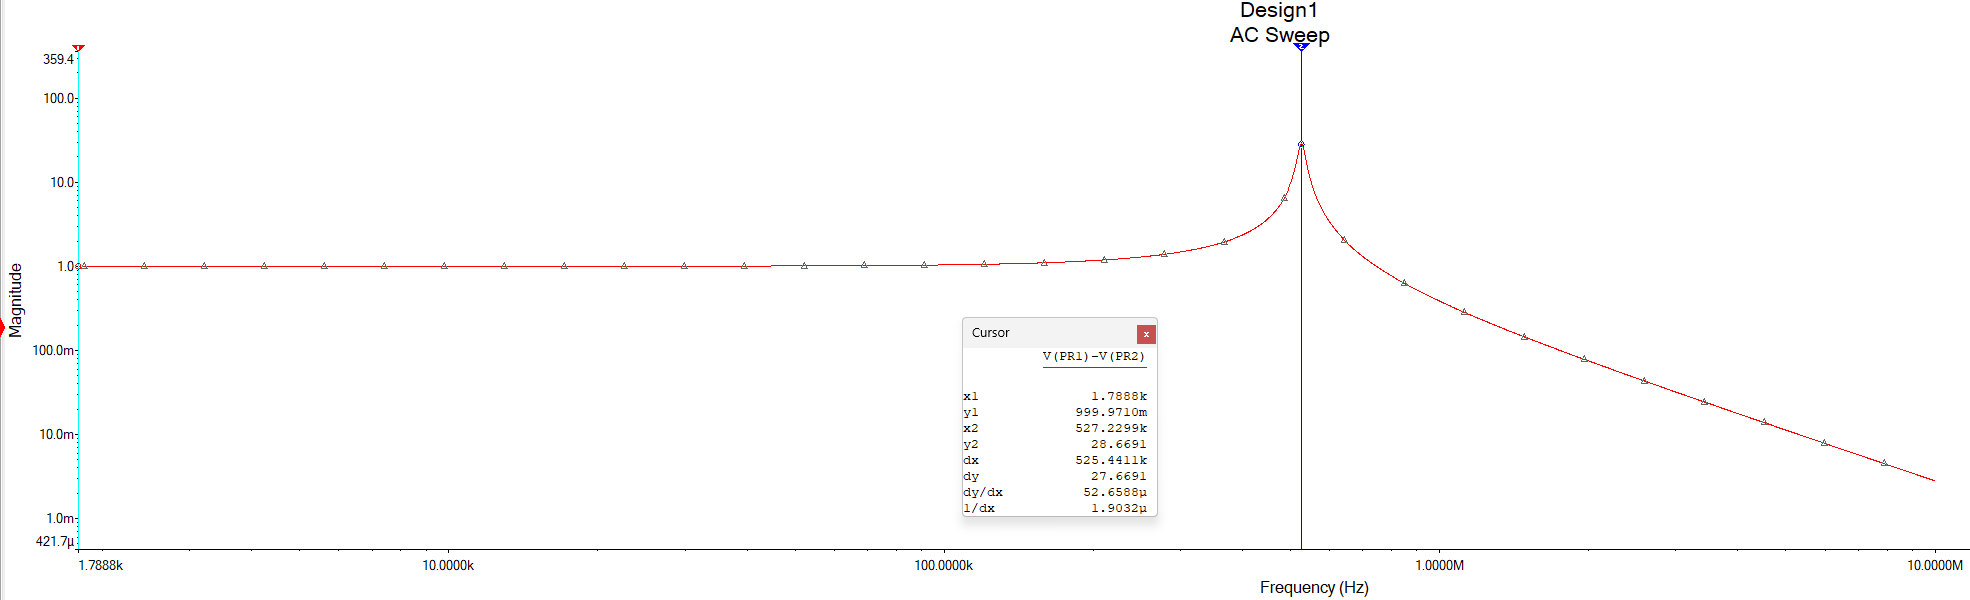
\includegraphics[width=1.0\textwidth]{fig_ac_20.png}
    \caption{AC Sweep，偏压 $V_d = 20\,\mathrm{V}$}
    \label{fig:ac_20}
\end{figure}

\section{数据处理与 $C_j$ 计算}

将仿真得到的不同偏压下的谐振频率 $f_0$ 代入公式 $C_j = \frac{1}{(2\pi f)^2 L}$ 计算结电容。

\subsection{MATLAB 处理代码}
\begin{lstlisting}[title=输入数据与 Cj 计算]
% 1. 输入测量数据
V_dc = [20, 15, 10, 5, 4 , 2, 1,  0.3]; 
f_res = [ 527229.9, 493173.8, 449779.9 ,384591.8,366437.6, 316956.7, 278612.1, 182810.0]; 

% 自动对齐长度
min_len = min(length(V_dc), length(f_res));
V_dc = V_dc(1:min_len);
f_res = f_res(1:min_len);

% 2. 计算 Cj (注意: L 修改为 0.01H)
L = 0.01; 
Cj = 1 ./ ((2 * pi * f_res).^2 * L);
Cj_inv_sq = 1 ./ (Cj.^2);

% 输出结果表
fprintf('电压(V)\t\t频率(Hz)\t\t电容(pF)\n');
for i = 1:length(V_dc)
    fprintf('%.1f V\t\t%.0f\t\t%.2f pF\n', V_dc(i), f_res(i), Cj(i)*1e12);
end
\end{lstlisting}

计算结果如下：
\begin{figure}[H]
    \centering
    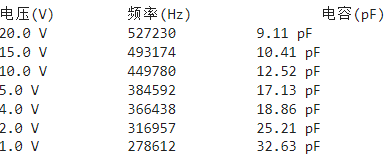
\includegraphics[width=0.7\textwidth]{f0.png}
    \caption{谐振频率下Cj计算结果}
    \label{fig:f0}
\end{figure}

\section{结果分析与绘图}

\subsection{$C_j - V_d$ 关系曲线}
由于在反向电压很小时（$0.3V$），二极管不稳定且接近导通，测量结果误差较大，因此在绘图和拟合时舍去最后一点数据。图 \ref{fig:cj} 展示了原始数据的连线趋势。

\begin{lstlisting}[title=Cj-Vd 绘图代码]
figure(2); 
% 舍去最后一个点 (0.3V)
if length(V_dc) > 1
    valid_idx = 1:length(V_dc)-1; 
else
    valid_idx = 1:length(V_dc);
end

% 数据排序，确保连线正确
[V_plot, sort_idx] = sort(V_dc(valid_idx)); 
Cj_plot = Cj(valid_idx(sort_idx));          

% 绘制散点与连线
scatter(V_plot, Cj_plot, 'bo', 'LineWidth', 1.5); hold on; 
plot(V_plot, Cj_plot, 'g-', 'LineWidth', 1.5);

xlabel("反向偏压 Vd (V)");
ylabel("结电容 Cj (F)");
title('Cj - Vd 关系图 (原始数据连线)');
grid on;
\end{lstlisting}

\begin{figure}[H]
    \centering
    % 请将 MATLAB Figure 2 保存为 fig_cj.png
    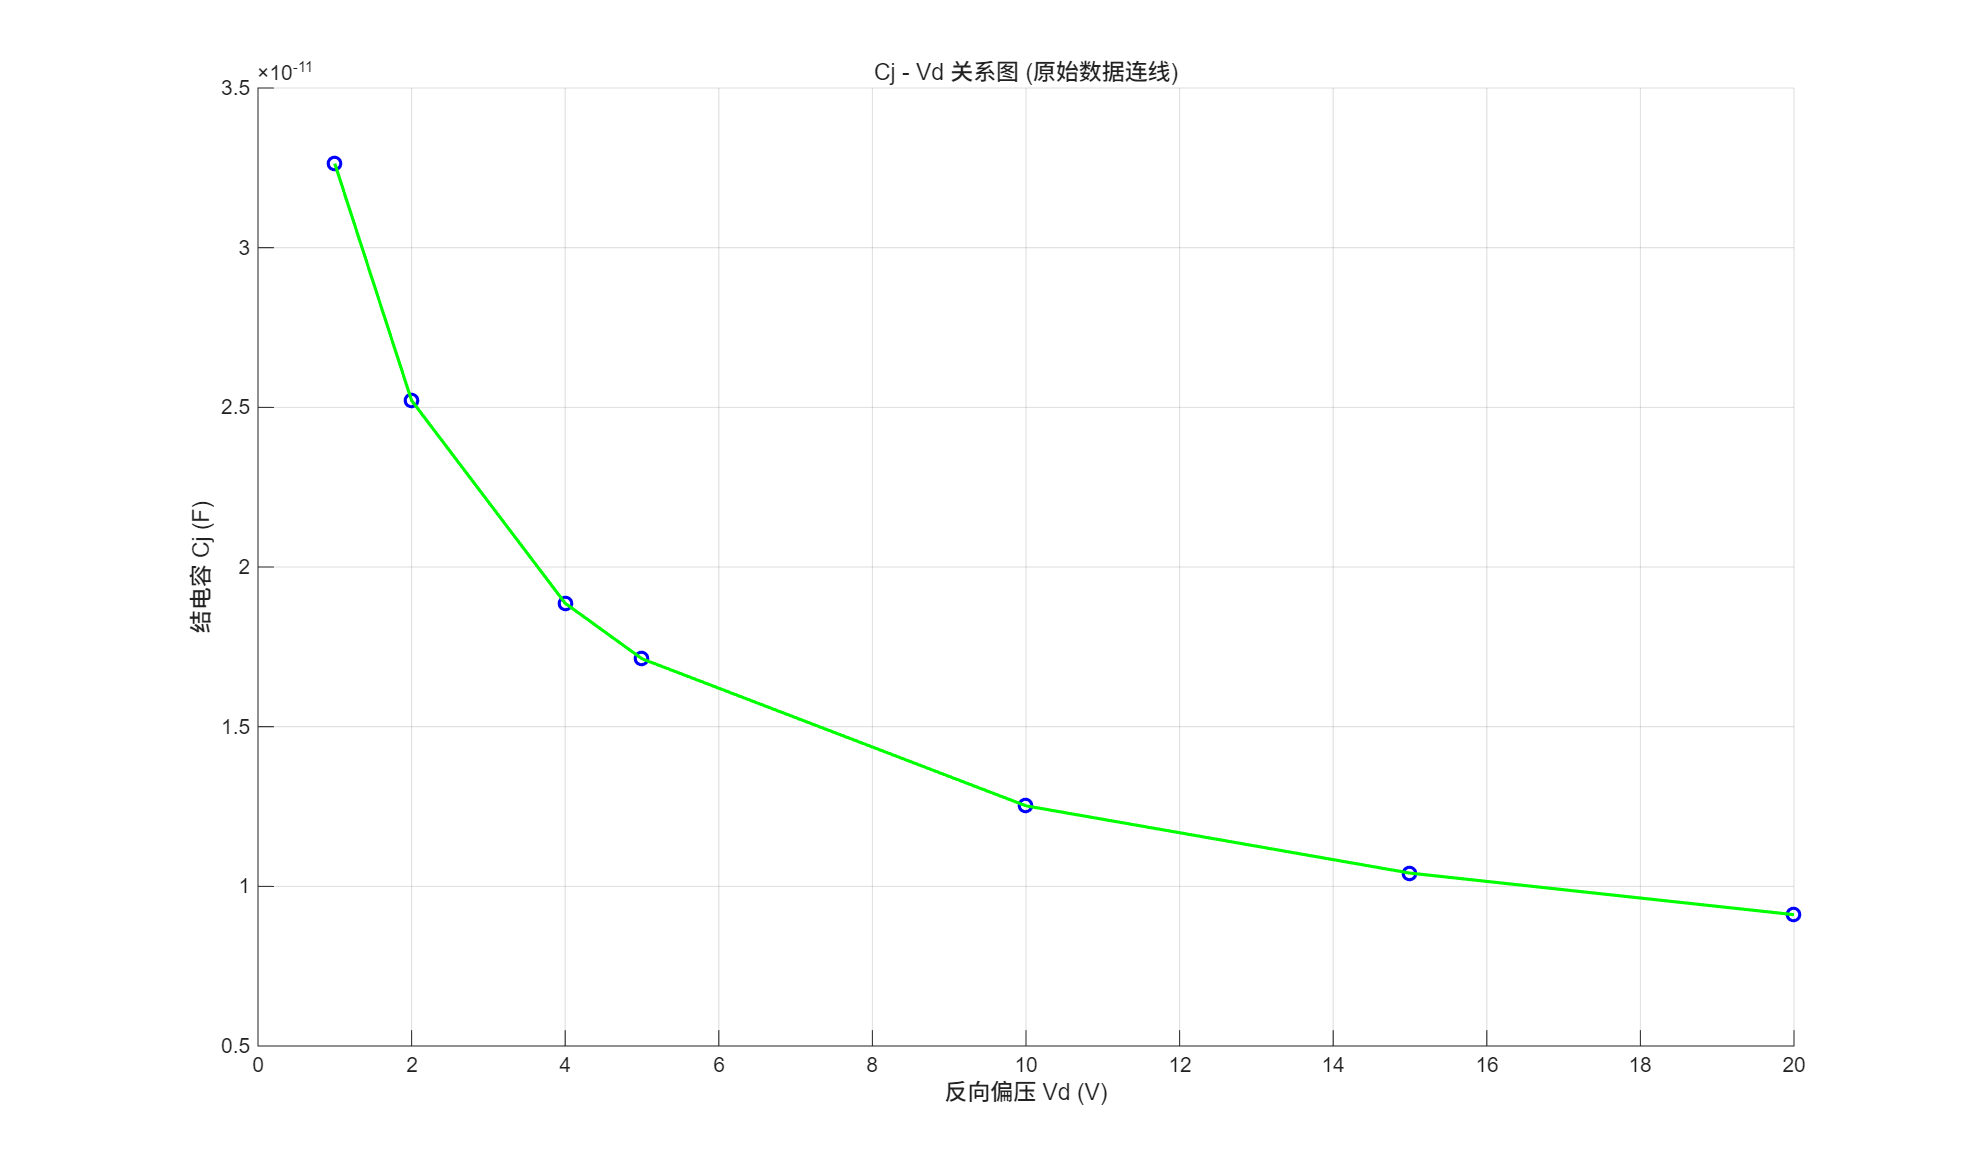
\includegraphics[width=0.7\textwidth]{fig_cj.png}
    \caption{$C_j - V_d$ 关系散点与连线图}
    \label{fig:cj}
\end{figure}

\subsection{$1/C_j^2 - V_d$ 线性拟合与 $C_{j0}$ 求取}
根据公式 $\frac{1}{C_j^2} = k(V_{bi} + V_R)$，通过线性拟合求取截距，从而计算零偏压结电容 $C_{j0}$。

\begin{lstlisting}[title=Cj0 拟合计算代码]
figure(3); 
Cj_inv_sq_plot = Cj_inv_sq(valid_idx(sort_idx)); 
scatter(V_plot, Cj_inv_sq_plot, 'ro', 'LineWidth', 2); hold on;

% 线性拟合
if length(V_plot) >= 2
    p2 = polyfit(V_plot, Cj_inv_sq_plot, 1);
    y_linear_line = polyval(p2, V_plot);
    plot(V_plot, y_linear_line, 'b-', 'LineWidth', 1.5);
=====================================Cj0_start=====================================
    intercept = p2(2); 
    Cj0 = sqrt(1 / intercept);
=====================================Cj0_end=====================================
    fprintf('线性拟合截距 b = %.4e\n', intercept);
    fprintf('零偏压结电容 Cj0 = %.2f pF\n', Cj0 * 1e12);
else
    fprintf('数据不足无法拟合\n');
end
xlabel("反向偏压 Vd (V)");
ylabel("1 / Cj^2");
title('线性拟合求 Cj0');
grid on;
\end{lstlisting}

\begin{figure}[H]
    \centering
    % 请将 MATLAB Figure 3 保存为 fig_linear.png
    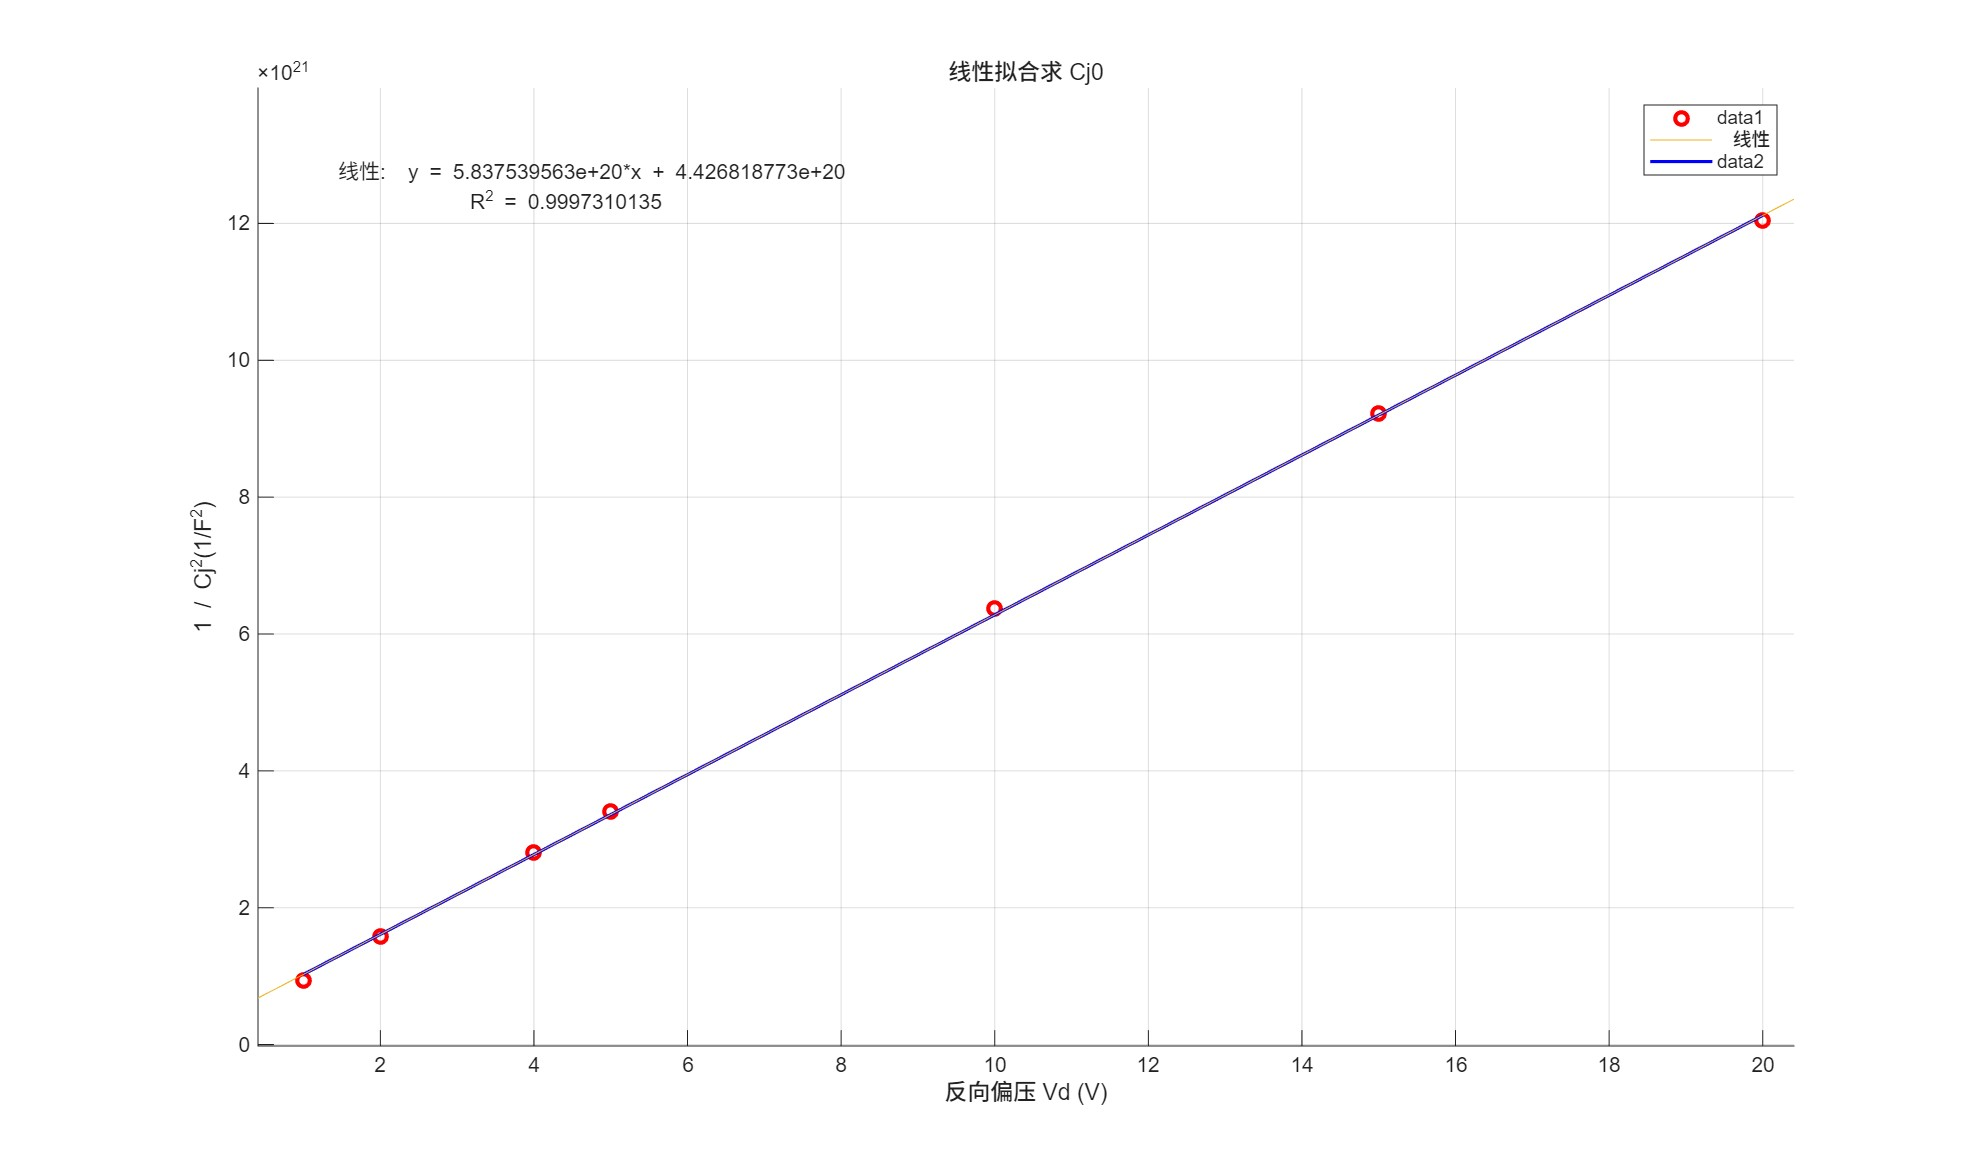
\includegraphics[width=0.7\textwidth]{fig_linear.jpg}
    \caption{$1/C_j^2 - V_d$ 线性拟合图}
    \label{fig:linear}
\end{figure}
计算得到$C_{j0} \approx 47.53 pF$。

\begin{figure}
    \centering
    % 请将 MATLAB Figure 3 保存为 fig_linear.png
    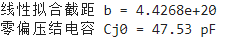
\includegraphics[width=0.3\textwidth]{bCj0.png}
    \caption{Cj0 计算结果展示}
    \label{fig:B and Cj0}
\end{figure}

\section{实验结论}

通过仿真实验与数据处理，我们验证了 PN 结电容随反向偏压增加而减小的特性。
\begin{itemize}
    \item 仿真中使用的电感值为 $L=10\text{mH}$。
    \item 通过线性拟合外推，计算得到的零偏压结电容 $C_{j0}$ 约为 \textbf{47.53} pF 。
\end{itemize}

\end{document}